\documentclass{standalone}
\usepackage{tikz}
\usetikzlibrary{patterns, positioning}

\begin{document}
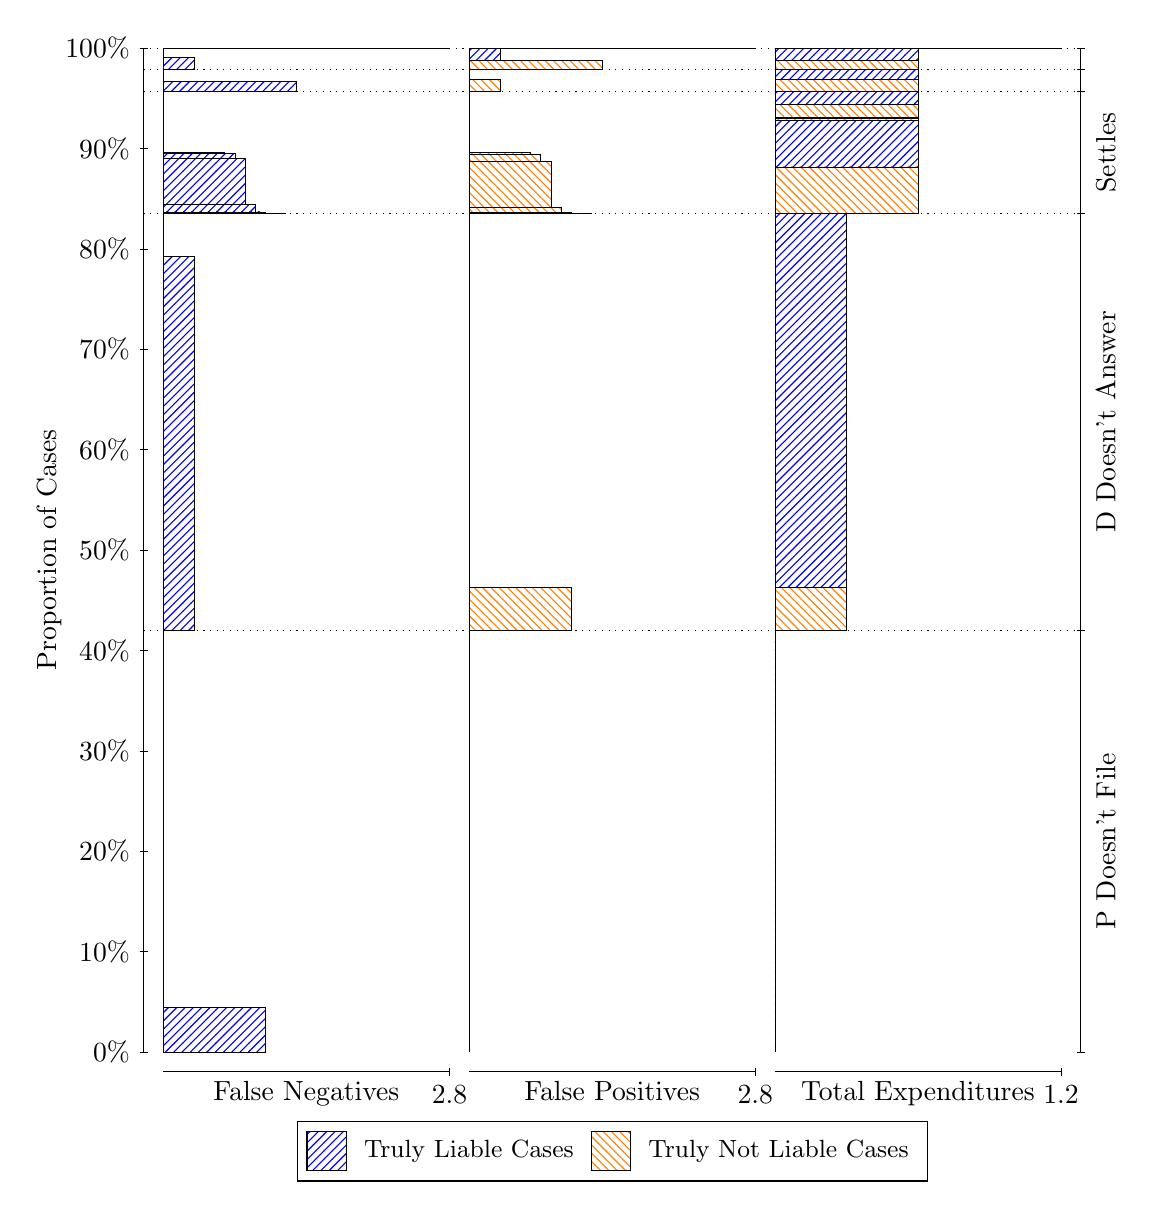
\begin{tikzpicture}
\draw[black, very thin] (1.5,1.75) -- (1.5,14.5);
\node[rotate=90, anchor=center] at (0.3, 8.125) {Proportion of Cases};
\draw[black, very thin] (1.45,1.75) -- (1.55,1.75);
\node[anchor=east] at (1.45, 1.75) {0\%};
\draw[black, very thin] (1.45,3.025) -- (1.55,3.025);
\node[anchor=east] at (1.45, 3.025) {10\%};
\draw[black, very thin] (1.45,4.3) -- (1.55,4.3);
\node[anchor=east] at (1.45, 4.3) {20\%};
\draw[black, very thin] (1.45,5.575) -- (1.55,5.575);
\node[anchor=east] at (1.45, 5.575) {30\%};
\draw[black, very thin] (1.45,6.85) -- (1.55,6.85);
\node[anchor=east] at (1.45, 6.85) {40\%};
\draw[black, very thin] (1.45,8.125) -- (1.55,8.125);
\node[anchor=east] at (1.45, 8.125) {50\%};
\draw[black, very thin] (1.45,9.4) -- (1.55,9.4);
\node[anchor=east] at (1.45, 9.4) {60\%};
\draw[black, very thin] (1.45,10.675) -- (1.55,10.675);
\node[anchor=east] at (1.45, 10.675) {70\%};
\draw[black, very thin] (1.45,11.95) -- (1.55,11.95);
\node[anchor=east] at (1.45, 11.95) {80\%};
\draw[black, very thin] (1.45,13.225) -- (1.55,13.225);
\node[anchor=east] at (1.45, 13.225) {90\%};
\draw[black, very thin] (1.45,14.5) -- (1.55,14.5);
\node[anchor=east] at (1.45, 14.5) {100\%};

\draw[black, very thin] (13.4,1.75) -- (13.4,14.5);
\draw[black, very thin] (13.35,1.75) -- (13.45,1.75);
\node[anchor=west] at (13.35, 1.75) {};
\draw[black, very thin] (13.35,7.104) -- (13.45,7.104);
\node[anchor=west] at (13.35, 7.104) {};
\draw[black, very thin] (13.35,12.399) -- (13.45,12.399);
\node[anchor=west] at (13.35, 12.399) {};
\draw[black, very thin] (13.35,13.949) -- (13.45,13.949);
\node[anchor=west] at (13.35, 13.949) {};
\draw[black, very thin] (13.35,14.229) -- (13.45,14.229);
\node[anchor=west] at (13.35, 14.229) {};
\draw[black, very thin] (13.35,14.494) -- (13.45,14.494);
\node[anchor=west] at (13.35, 14.494) {};
\draw[black, very thin] (13.35,14.495) -- (13.45,14.495);
\node[anchor=west] at (13.35, 14.495) {};
\draw[black, very thin] (13.35,14.5) -- (13.45,14.5);
\node[anchor=west] at (13.35, 14.5) {};

\draw[black, very thin, pattern color=blue, pattern=north east lines] (1.75,1.75) rectangle (3.0476,2.3174);
\draw[black, very thin, pattern color=orange, pattern=north west lines] (1.75,2.3174) rectangle (1.75,7.104);
\draw[black, very thin, pattern color=blue, pattern=north east lines] (1.75,7.104) rectangle (2.1393,11.856);
\draw[black, very thin, pattern color=orange, pattern=north west lines] (1.75,11.856) rectangle (1.75,12.399);
\draw[black, very thin, pattern color=blue, pattern=north east lines] (1.75,12.399) rectangle (3.3071,12.399);
\draw[black, very thin, pattern color=blue, pattern=north east lines] (1.75,12.399) rectangle (3.1774,12.4);
\draw[black, very thin, pattern color=blue, pattern=north east lines] (1.75,12.4) rectangle (3.0476,12.418);
\draw[black, very thin, pattern color=blue, pattern=north east lines] (1.75,12.418) rectangle (2.9179,12.418);
\draw[black, very thin, pattern color=blue, pattern=north east lines] (1.75,12.418) rectangle (2.9179,12.515);
\draw[black, very thin, pattern color=blue, pattern=north east lines] (1.75,12.515) rectangle (2.7881,13.095);
\draw[black, very thin, pattern color=blue, pattern=north east lines] (1.75,13.095) rectangle (2.6583,13.161);
\draw[black, very thin, pattern color=blue, pattern=north east lines] (1.75,13.161) rectangle (2.5286,13.174);
\draw[black, very thin, pattern color=blue, pattern=north east lines] (1.75,13.174) rectangle (2.3988,13.175);
\draw[black, very thin, pattern color=blue, pattern=north east lines] (1.75,13.175) rectangle (2.269,13.176);
\draw[black, very thin, pattern color=orange, pattern=north west lines] (1.75,13.176) rectangle (1.75,13.949);
\draw[black, very thin, pattern color=blue, pattern=north east lines] (1.75,13.949) rectangle (3.4369,14.073);
\draw[black, very thin, pattern color=orange, pattern=north west lines] (1.75,14.073) rectangle (1.75,14.229);
\draw[black, very thin, pattern color=blue, pattern=north east lines] (1.75,14.229) rectangle (2.1393,14.379);
\draw[black, very thin, pattern color=orange, pattern=north west lines] (1.75,14.379) rectangle (1.75,14.494);
\draw[black, very thin, pattern color=blue, pattern=north east lines] (1.75,14.494) rectangle (5.3833,14.495);
\draw[black, very thin, pattern color=orange, pattern=north west lines] (1.75,14.495) rectangle (1.75,14.495);
\draw[black, very thin, pattern color=orange, pattern=north west lines] (1.75,14.495) rectangle (1.75,14.496);
\draw[black, very thin, pattern color=blue, pattern=north east lines] (1.75,14.496) rectangle (1.75,14.5);
\draw[black, very thin, pattern color=orange, pattern=north west lines] (5.6333,1.75) rectangle (5.6333,6.5366);
\draw[black, very thin, pattern color=blue, pattern=north east lines] (5.6333,6.5366) rectangle (5.6333,7.104);
\draw[black, very thin, pattern color=orange, pattern=north west lines] (5.6333,7.104) rectangle (6.931,7.6469);
\draw[black, very thin, pattern color=blue, pattern=north east lines] (5.6333,7.6469) rectangle (5.6333,12.399);
\draw[black, very thin, pattern color=orange, pattern=north west lines] (5.6333,12.399) rectangle (7.1905,12.4);
\draw[black, very thin, pattern color=orange, pattern=north west lines] (5.6333,12.4) rectangle (7.0607,12.4);
\draw[black, very thin, pattern color=orange, pattern=north west lines] (5.6333,12.4) rectangle (6.931,12.411);
\draw[black, very thin, pattern color=orange, pattern=north west lines] (5.6333,12.411) rectangle (6.8012,12.476);
\draw[black, very thin, pattern color=orange, pattern=north west lines] (5.6333,12.476) rectangle (6.6714,13.056);
\draw[black, very thin, pattern color=orange, pattern=north west lines] (5.6333,13.056) rectangle (6.5417,13.152);
\draw[black, very thin, pattern color=orange, pattern=north west lines] (5.6333,13.152) rectangle (6.4119,13.172);
\draw[black, very thin, pattern color=orange, pattern=north west lines] (5.6333,13.172) rectangle (6.2821,13.172);
\draw[black, very thin, pattern color=orange, pattern=north west lines] (5.6333,13.172) rectangle (6.1524,13.172);
\draw[black, very thin, pattern color=blue, pattern=north east lines] (5.6333,13.172) rectangle (5.8929,13.173);
\draw[black, very thin, pattern color=blue, pattern=north east lines] (5.6333,13.173) rectangle (5.7631,13.175);
\draw[black, very thin, pattern color=blue, pattern=north east lines] (5.6333,13.175) rectangle (5.6333,13.949);
\draw[black, very thin, pattern color=orange, pattern=north west lines] (5.6333,13.949) rectangle (6.0226,14.105);
\draw[black, very thin, pattern color=blue, pattern=north east lines] (5.6333,14.105) rectangle (5.6333,14.229);
\draw[black, very thin, pattern color=orange, pattern=north west lines] (5.6333,14.229) rectangle (7.3202,14.344);
\draw[black, very thin, pattern color=blue, pattern=north east lines] (5.6333,14.344) rectangle (6.0226,14.494);
\draw[black, very thin, pattern color=orange, pattern=north west lines] (5.6333,14.494) rectangle (5.6333,14.495);
\draw[black, very thin, pattern color=blue, pattern=north east lines] (5.6333,14.495) rectangle (5.6333,14.495);
\draw[black, very thin, pattern color=orange, pattern=north west lines] (5.6333,14.495) rectangle (9.2667,14.496);
\draw[black, very thin, pattern color=blue, pattern=north east lines] (5.6333,14.496) rectangle (7.969,14.5);
\draw[black, very thin, pattern color=orange, pattern=north west lines] (9.5167,1.75) rectangle (9.5167,6.5366);
\draw[black, very thin, pattern color=blue, pattern=north east lines] (9.5167,6.5366) rectangle (9.5167,7.104);
\draw[black, very thin, pattern color=orange, pattern=north west lines] (9.5167,7.104) rectangle (10.425,7.6469);
\draw[black, very thin, pattern color=blue, pattern=north east lines] (9.5167,7.6469) rectangle (10.425,12.399);
\draw[black, very thin, pattern color=orange, pattern=north west lines] (9.5167,12.399) rectangle (11.333,12.99);
\draw[black, very thin, pattern color=blue, pattern=north east lines] (9.5167,12.99) rectangle (11.333,13.585);
\draw[black, very thin, pattern color=orange, pattern=north west lines] (9.5167,13.585) rectangle (11.333,13.605);
\draw[black, very thin, pattern color=blue, pattern=north east lines] (9.5167,13.605) rectangle (11.333,13.624);
\draw[black, very thin, pattern color=orange, pattern=north west lines] (9.5167,13.624) rectangle (11.333,13.786);
\draw[black, very thin, pattern color=blue, pattern=north east lines] (9.5167,13.786) rectangle (11.333,13.949);
\draw[black, very thin, pattern color=orange, pattern=north west lines] (9.5167,13.949) rectangle (11.333,14.105);
\draw[black, very thin, pattern color=blue, pattern=north east lines] (9.5167,14.105) rectangle (11.333,14.229);
\draw[black, very thin, pattern color=orange, pattern=north west lines] (9.5167,14.229) rectangle (11.333,14.344);
\draw[black, very thin, pattern color=blue, pattern=north east lines] (9.5167,14.344) rectangle (11.333,14.494);
\draw[black, very thin, pattern color=orange, pattern=north west lines] (9.5167,14.494) rectangle (13.15,14.495);
\draw[black, very thin, pattern color=blue, pattern=north east lines] (9.5167,14.495) rectangle (13.15,14.495);
\draw[black, very thin, pattern color=orange, pattern=north west lines] (9.5167,14.495) rectangle (13.15,14.496);
\draw[black, very thin, pattern color=blue, pattern=north east lines] (9.5167,14.496) rectangle (13.15,14.5);
\draw[black, dotted] (1.5,7.104) -- (13.4,7.104);
\draw[black, dotted] (1.5,12.399) -- (13.4,12.399);
\draw[black, dotted] (1.5,13.949) -- (13.4,13.949);
\draw[black, dotted] (1.5,14.229) -- (13.4,14.229);
\draw[black, dotted] (1.5,14.494) -- (13.4,14.494);
\draw[black, dotted] (1.5,14.495) -- (13.4,14.495);
\draw[black, very thin] (1.75,1.5) -- (5.3833,1.5);
\node[anchor=north] at (3.5667, 1.5) {False Negatives};
\draw[black, very thin] (5.3833,1.45) -- (5.3833,1.55);
\node[anchor=north] at (5.3833, 1.45) {2.8};

\draw[black, very thin] (5.6333,1.5) -- (9.2667,1.5);
\node[anchor=north] at (7.45, 1.5) {False Positives};
\draw[black, very thin] (9.2667,1.45) -- (9.2667,1.55);
\node[anchor=north] at (9.2667, 1.45) {2.8};

\draw[black, very thin] (9.5167,1.5) -- (13.15,1.5);
\node[anchor=north] at (11.333, 1.5) {Total Expenditures};
\draw[black, very thin] (13.15,1.45) -- (13.15,1.55);
\node[anchor=north] at (13.15, 1.45) {1.2};

\node[black, centered, rotate=90] at (13.72, 4.427) {P Doesn't File};
\node[black, centered, rotate=90] at (13.72, 9.7517) {D Doesn't Answer};
\node[black, centered, rotate=90] at (13.72, 13.174) {Settles};





\draw (7.449999999999999,1.5) node[draw=none] (baseCoordinate) {};
\begin{scope}[align=center]
        \matrix[scale=0.5, draw=black, below=0.5cm of baseCoordinate, nodes={draw}, column sep=0.1cm]{
            \node[rectangle, draw, minimum width=0.5cm, minimum height=0.5cm, pattern=north east lines, pattern color=blue] {}; &
            \node[draw=none, font=\small] (B) {Truly Liable Cases}; &
            \node[rectangle, draw, minimum width=0.5cm, minimum height=0.5cm, pattern=north west lines, pattern color=orange] {}; &
            \node[draw=none, font=\small] (B) {Truly Not Liable Cases}; \\
            };
\end{scope}

\end{tikzpicture}
\end{document}